\documentclass[tikz = true, border=0mm]{standalone}
\usepackage{tikz}
\usetikzlibrary{positioning}
\usetikzlibrary{arrows,shapes}
\usepackage{fontspec}
\setmainfont{Equity Text A}[SmallCapsFont={Equity Caps A}]
\definecolor{firebrick4}{HTML}{8B1A1A}
\definecolor{royalblue4}{RGB}{39,64,139}
\definecolor{myviolet}{HTML}{51315E}

\begin{document}
	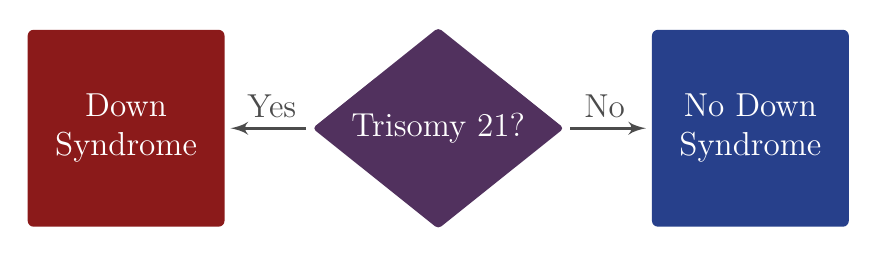
\begin{tikzpicture}
    [node distance=1.1cm and 1.1cm,
    post/.style={->,
    	         black!70,
    	         shorten >=2pt,
    	         shorten <=2pt,
    	         >=latex', 
    	         very thick, 
    	         font=\large}, 
    ob/.style={rectangle,
    	       inner sep=1mm,
    	       minimum width=2.5cm, 
    	       minimum height=2.5cm, 
    	       rounded corners=0.75mm,
    	       font=\large, 
    	       text = white}]
    \node[shape=diamond, 
          fill=myviolet,
          rounded corners=0.5mm,
          shape aspect=1.25, 
          text = white, 
          font = \large] (Trisomy) at (0,0) {Trisomy 21?};
    \node [ob,
           fill=firebrick4,
           left=of Trisomy,
           align=center] (Down) {Down\\Syndrome};
    \node [ob,
          fill=royalblue4, 
          right=of Trisomy, 
          align=center] (NoDown) {No Down\\Syndrome}; 
    \draw[post] (Trisomy) -- (Down) node [pos=.46,above] {Yes};
    \draw[post] (Trisomy) -- (NoDown) node [pos=.46,above] {No};
\end{tikzpicture}
\end{document}